\chapter{Implementation}
% (more or less telling whats in my code; implementation details; describing dataset; which network and which hyper parameters do I use; how does the application look like)
\section{Setup}

In order to conduct the training process described by the methods used in the previous chapter, it was necessary to have a computer with a powerful GPU in order to speed up training. For this Master thesis, the experiments/training were conducted on a Nvidia Titan X (Pascal) GPU with 12 GB of memory. 
\newline\newline
The framework used for Machine Learning was TensorFlow. It provides a specific software package for GPU usage which was called 'tensorflow-gpu' and was installed in version '1.14.0'. Furthermore, Keras was used on top of Tensorflow, which was a neural network library that made it faster and easier to interact with the underlying Machine Learning framework. Keras version used was 2.2.5.
\newline\newline
Further important third-party software packages include:
\begin{itemize}
    \item Keras-VggFace: Version 0.6
    \item MTCNN:         Version 0.1.0
    \item OpenCV:        Version 4.1
\end{itemize}
All these frameworks and packages were used inside the Python programming language. The utilized version was 3.6.


\section{Dataset}
\textbf{Background}
\newline
The selected AFEW-VA dataset \citet{Kossaifi:2017:AFEW-VADatabase} is based upon the Acted Facial Expressions In-The-Wild database (AFEW) proposed in \citeyear{Dhall:2012:AFEW} by \citet{Dhall:2012:AFEW}. The AFEW dataset is composed of video clips that try to depict a real-world environment. It captures facial expressions, natural head pose movements, occlusions, subjects' races, gender, diverse ages, and multiple subjects in a scene. The authors labeled the video clips with one of six basic expressions: anger, disgust, fear, happiness, sadness, surprise, or neutral.
\newline\newline
The AFEW-VA dataset \citep{Kossaifi:2017:AFEW-VADatabase} uses the same underlying real-world video data, but it did not annotate its video clips with one of six basic expressions. Instead it used the two dimensional affective space with valence and arousal. While valence expressed how positive or negative an emotion is, arousal expresses how strong or weak an emotion is.
\newline\newline
Furthermore, as the name of the dataset already suggests, the dataset is compopsed of data that was collected under 'In-The-Wild' conditions. 'In-The-Wild' refers to real-life conditions in video clips, which make it very difficult to recognize emotions. \citet{Salah:2018:VideoBasedER} explained that these difficulties can be caused by, for example, uncontrolled illumination or uncontrolled video quality due to a different recording medium, like webcams by individuals vs. professional cameras. Such 'In-The-Wild' data is usually acquired from talk shows, movies or other naturalistic interactions. 
\newline\newline
As the research conducted during this Master thesis is intended to serve as a basis for a further real-life application in video-call scenarios, it was clear that the dataset needed to be as close to 'In-The-Wild' conditions as possible. Furthermore, it was decided that it was more important to capture as much of an emotion's information as possible rather than placing value on the interpretation of emotions. As a result, the AFEW-VA dataset got chosen because of its 'In-the-Wild' conditions, its 2D Affective Space model for emotion representation and its backing by the scientific community when it comes to providing comparable results.
\newline\newline
\textbf{Data structure}\newline
The dataset is split into 600 folders, each representing a different video clip. Each video clip is taken from a different subject. Each of these folders holds multiple frames which together make up the video clip. Moreover, the folder also holds a .json file which holds the label for each frame and describes it in terms of valence, arousal and landmark points.
\newline\newline
This .json file contains for each frame a value for the valence and another value for the arousal. Both values have an annotation level ranging from -10 to +10 in full integer values. This results in a total of 21 levels.\citep{Kossaifi:2017:AFEW-VADatabase} Additionally, the file also includes pre-labeled landmarks for face detection purposes. However, these landmarks were not utilized in the training of the proposed model, as third-party modules were being used for performing face detection and landmark determination tasks.
\newline\newline
\textbf{Benchmark}
\newline
In order to objectively compare the results from the original AFEW-VA paper proposed by \citet{Kossaifi:2017:AFEW-VADatabase}, it was essential to lay out the circumstances under which the results were obtained. In the case of the AFEW-VA paper \citep{Kossaifi:2017:AFEW-VADatabase}, as well as the simulatenous VA prediction paper \citep{Handrich:2020:SimultaneousPredVA}, the data got divided in 5 disjoint folds in a subject-independent manner, meaning a subject did not appear in different folds. Subsequently, they performed a 5-fold-cross-validation for the prediction of valence and arousal values for each frame of a video clip.\citep{Kossaifi:2017:AFEW-VADatabase}
\newline\newline
\citet{Roehrich:2020:TrainValidateTest} argued that when comparing different models it is not enough to use a training and a testing set, as it might still be possible that one model is better than the other due to randomness during the training process. Thus, in addition to the above-mentioned approach of creating 5 folds in a subject independent manner, it was important to separate the folds into training, validation and testing subsets. The split of the database into subsets is shown in figure \ref{fig:TrainTestSplit} and these subsets fulfill the following purposes:

\begin{itemize}
    \item The training dataset will be used for the actual training of the model
    \item The validation dataset is used for testing during the training process. Thus, it serves as a metric that needs to be improved by, for example, adapting the model architecture. Moreover, it serves as the metric for the EarlyStopping mechanism which ends the training process when the observed metric stales in its performance
    \item The testing dataset is all about the actual measurement of the model's performance on a third previously unseen dataset
\end{itemize}

\begin{figure}[H]
  \begin{center}
  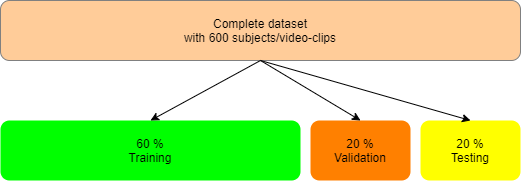
\includegraphics[angle=0, width=0.6\textwidth]{Figures/TrainTest_Split.png}
  \caption{Train, Validation and Test split}
  \label{fig:TrainTestSplit}
  \end{center}
\end{figure}

For the final results of the proposed approach, 5-fold-cross-validation was conducted by splitting the 600 subjects/video-clips into five folds with each containing 120 subjects. Four out of those five folds were used for training, while one fold was reserved for the evaluation of the model after the finished training. The four folds were again split into training and validation, with one fold serving as the validation set. This approach can also be seen in figure \ref{fig:CrossValidationSplit}.

\begin{figure}[H]
  \begin{center}
  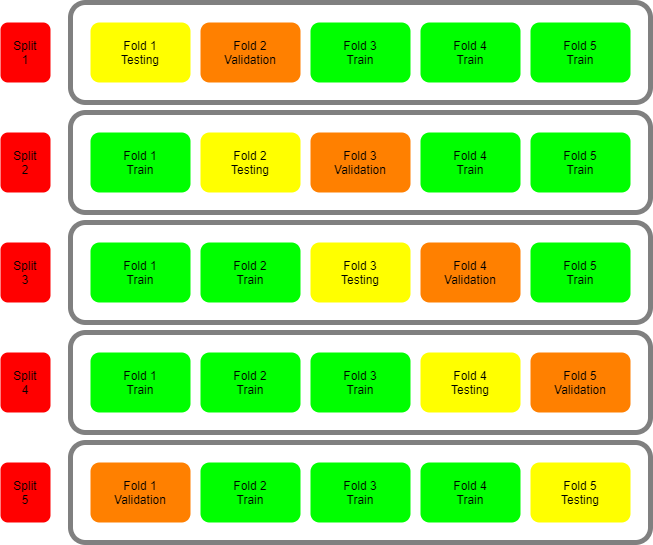
\includegraphics[angle=0, width=0.8\textwidth]{Figures/CrossValidation_Split.png}
  \caption{Cross-Validation split}
  \label{fig:CrossValidationSplit}
  \end{center}
\end{figure}

This approach ensured that there was no overlap in terms of subjects between the training and testing/evaluation. Therefore, the subset for the evaluation of the model performance contained only frames from subjects that were previously not seen by the model during the training process.

% \begin{quote}
%     To compare the performance of various features, we sampled regularly an equal number of frames from each sequence to obtain a set of frames representative of the whole dataset, which we then divided in 5 disjoint folds in a subject-independent manner (i.e. a subject does not appear in two different folds). We then performed a 5-fold cross-validation (i.e. we iteratively used one of the set for testing and the other 4 for training) to predict the valence and arousal values for each frame. \citep{Kossaifi:2017:AFEW-VADatabase}
% \end{quote}

\section{Architecture}

\begin{figure}[H]
  \begin{center}
  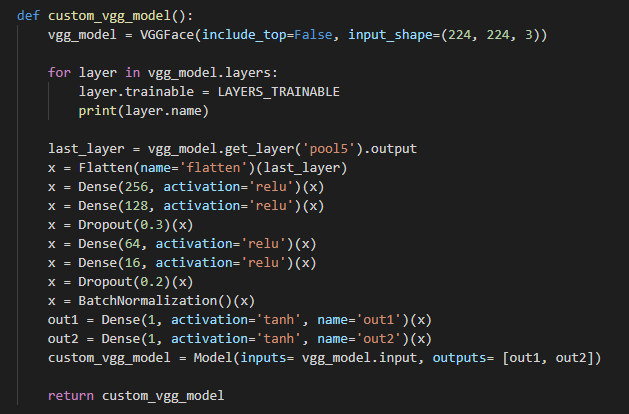
\includegraphics[angle=0, width=1.0\textwidth]{Figures/model_architecture.PNG}
  \caption{Neural Network Architecture}
  \label{fig:NNArchitecture}
  \end{center}
\end{figure}

Figure \ref{fig:NNArchitecture} describes the architecture of the neural network with the following elements:

\begin{itemize}
    \item Line \#2: the pre-trained VGGFace model is being loaded with 'resnet50' as its neural network architecture. With the parameter 'include\_top' set to False allows to exclude the classifier of th pre-trained network on face detection.
    \item Line \#5 to line \#10: The VGGFace model is set to trainable or non-trainable. For the first three epochs of fune-tuning, the model gets set to non-trainable. Afterwards it is set to trainable, and allows the model to update its weights.
    \item Line \#12: The output of the VGGFace model is being accessed in in line \#13 reduced in dimensionality in order to fit the input requirements for the following layer.
    \item Line \#15 to line \#18 contains the classifier consisting of a Dense layer (1024 units), together with two Dropout and a Batch Normalization layer in order to improve generalization capabilities.
    \item Line \#20 and \#21: The output for each evaluation metric is defined individually. This separation makes it possible to neatly visualize the outcomes and the 'tanh' activation resized the output to a floating-point number range of -1 to +1.
\end{itemize}

The choice of only using a single Dense layer in the block of fully connected layers was based on a paper \citep{Pittaras:2017:FineTuningStrategiesComparison} that compared different fine-tuning strategies on pre-trained neural networks which could show that
\begin{quote}
    increasing the depth of a pre-trained network with one more fully-connected layer and fine-tuning the rest of the layers on the target dataset can improve the network’s concept detection accuracy compared to other fine-tuning approaches. \citep[~p. 103]{Pittaras:2017:FineTuningStrategiesComparison}
\end{quote}

Moreover, \citet{Pittaras:2017:FineTuningStrategiesComparison} could obtained their best results with a fine-tuning approach that replaced the pre-trained classifier of a network with a single Dense layer containing a high number of neurons.

%%%%%%%%%%%%%%%%%%%%%%%%%%%%%%%%%%%%%%%%%%%%%%%%%%%%%%%%%


\section{Fine-tuning}
\subsubsection{ResNet50 model}
ResNet50, short for Residual Network, is a very deep neural network architecture that was invented for the purpose of image classification, resulting in winning the ImageNet challenge in 2015. \citep{Dwivedi:2019:ResNetInKeras}

\begin{figure}[H]
  \begin{center}
  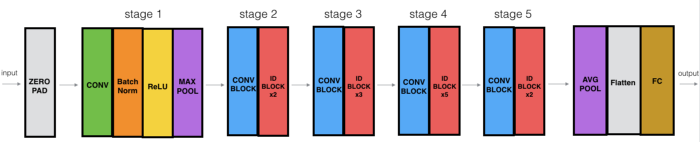
\includegraphics[angle=0, width=1.0\textwidth]{Figures/resnet50.png}
  \caption{ResNet50 Architecture \citep{Dwivedi:2019:ResNetInKeras}}
  \label{fig:ResNet50Architecture}
  \end{center}
\end{figure}

\begin{quote}
    The ResNet-50 model consists of 5 stages each with a convolution and Identity block. Each convolution block has 3 convolution layers and each identity block also has 3 convolution layers. The ResNet-50 has over 23 million trainable parameters. \citep[~para. 14]{Dwivedi:2019:ResNetInKeras}
\end{quote}

ResNet50 is defined by a very deep-layered neural network which traditionally posed a difficult challenge to researchers, as the training process gets worse the deeper the neural network due to the notorious vanishing gradient problem. The vanishing gradient leads to a rapid saturation of the model's weights which results in a degradation of the overall model performance. To fight this problem, ResNet introduced a novel concept, named skip connection, where the results of a block are added together with the original input before applying an activation function. \citep{Dwivedi:2019:ResNetInKeras}
\newline\newline
This concept is also illustrated in the following figure \ref{fig:ResNet50IdentityBlock} for the an identity block:

\begin{figure}[H]
  \begin{center}
  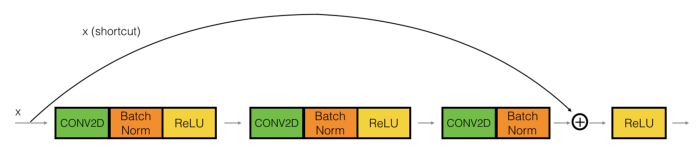
\includegraphics[angle=0, width=0.9\textwidth]{Figures/ResNet50_IdentityBlock.png}
  \caption{ResNet50 Identity Block\citep{Dwivedi:2019:ResNetInKeras}}
  \label{fig:ResNet50IdentityBlock}
  \end{center}
\end{figure}

This operation is however, only possible when the two inputs for the addition have the same shape. Due to the layout of the ResNet50 architecture, this is inherently the case for the Identity Block. For the Convolution Block a further operation is needed to transform the block's original input into the same shape as the outcome of the Convolutional layers. As can be seen in figure \ref{fig:ResNet50ConvBlock}, this was done by applying a separate Convolutional plus Batch Normalization layer to the original input and choosing its hyperparameters in a way that the output will be in the same shape as the outcome of the Convolutional layers.

\begin{figure}[H]
  \begin{center}
  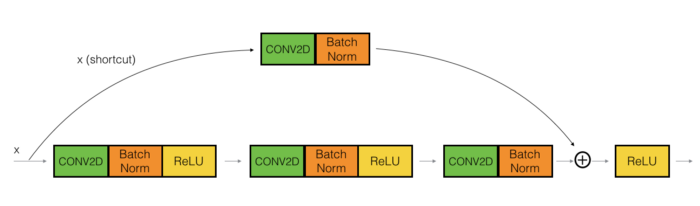
\includegraphics[angle=0, width=0.9\textwidth]{Figures/ResNet50_ConvBlock.png}
  \caption{ResNet50 Convolutional Block\citep{Dwivedi:2019:ResNetInKeras}}
  \label{fig:ResNet50ConvBlock}
  \end{center}
\end{figure}

\citet{Dwivedi:2019:ResNetInKeras} argued that this approach is helpful in mitigating the problem of vanishing gradients, as its skip connection concepts, firstly, provided an alternate shortcut path for gradients to flow through and secondly, ensured that the subsequent block will perform at least as well as the previous.

\subsubsection{Pre-trained network}
As recommended by \citet{Chollet:2017:DeepLearningPython} using a pre-trained neural network is a highly effective approach to deep learning on a small image dataset. The AFEW-VA dataset with its 30.000 frames (= 600 video clips) can be considered a rather small dataset \citep{Kossaifi:2017:AFEW-VADatabase}.

\begin{quote}
    A pretrained network is a saved network that was previously trained on a large dataset, typically on a large-scale image-classification task. If this original dataset is large enough and general enough, then the spatial hierarchy of features learned by the pretrained network can effectively act as a generic model of the visual world, and hence its features can prove useful for many different Computer Vision problems, even though these new problems may involve completely different classes than those of the original task. \citep[~p. 143]{Chollet:2017:DeepLearningPython}
\end{quote}

\citet{Chollet:2017:DeepLearningPython} further elaborated that using a pre-trained network for small-data problems makes deep learning a very effective approach due to its portability of learned features across different problems.
\newline\newline
This is why, it seemed promising to solve the Emotion Recognition challenge at hand with a neural network that was pre-trained on a more general and holistic dataset. Therefore, a ResNet50 neural network architectur, pre-trained on a large-scale face recognition dataset containing 3.31 million images, called VGGFace2 \citep{Cao:2018:VGGFace2} was used.


\subsubsection{Fine-tuning strategy}
The layers inside a deep neural network are commonly divided into the convolutional base and the classifier. In the proposed approach, the ResNet50 architecture served as the convolutional base, while the classifier was added by manually defining the respective layers. The convolutional base was initialized with its pre-trained weights, while the classifier wasn't yet trained.
\newline\newline
The exact steps for fine-tuning a neural network were summarized by \citet{Chollet:2017:DeepLearningPython} as follows:
\begin{enumerate}
    \item Add your custom network on top of an already-trained base network
    \item Freeze the base network
    \item Train the part you added
    \item Unfreeze some layers in the base network
    \item Jointly train both these layers and the part you added
\end{enumerate}

\citet{Chollet:2017:DeepLearningPython} further highlighted that if the classifier isn't already trained and the whole model, including the pre-trained convolutional base, gets fine-tuned, the error being propagated through the network will be too big. This might result in the destruction of previously learned representations by the layers. As a result, the custom network part (in the case of the here proposed approach: the classifier) needed to be trained first separately as mentioned in step 3. 
\newline\newline
As mentioned in step 4 only some layers of the base network were unfrozen and thus, used during training. According to \citet{Chollet:2017:DeepLearningPython}, it is more useful to fine-tune the higher layers because these encode more specialized features and need to be readjusted to the new problem. Fine-tuning all the layers was theoretically possible, although it would have increased the risk of overfitting. Therefore, it was better to keep the lower layers of the convolutional base frozen as they encoded more generic features which can be useful for a wide variety of tasks/problems.


% \citet{Yan:2016:MultiClueFusion} made use of multi clue fusion to further enhance the accuracy of an emotion recognition in the Wild. They showed that with using only the VGGFace model as a predictor for the Emotion Recognition challenge, they got a surprisingly high accuracy of about 36 per cent. They also mention that it the model will perform better as they recognize emotions over multiple frames and conduct fine-tuning on the VGGFace model. (Fintuning = the adaption of a pre-trained model to the current challenge, usually done together with a new dataset)
% \newline\newline
% Furthermore, they detect faces with Single Shot Detector (SSD) and whenever it fails, they crop the image manually so far, that the detector "has" to detect it. However, in the approach describe in this thesis, images with a non-detectable face will be passed into the model in their original size. Thus, no manual cropping is being conducted. Additionally, they focus on the concept of action units (AU) together with landmarks. They define a facial expression is a combination of several action units (AU) movements, with the action units being the trajectories of vital facial
% landmarks.
% \citep{Yan:2016:MultiClueFusion}

%%%%%%%%%%%%%%%%%%%%%%%%%%%%%%%%%%%%%%%%%%%%%%%%%%%%%%%%%

\section{Metrics}
Metrics, in Machine Learning, are used to evaluate the performance of a Neural Network. Probably the most widely-used metric is 'accuracy' which tells you about the share of correctly predicted data points. 
\newline\newline
As the present challenge of predicting values for valence and arousal is better solved through regression, the 'accuracy' metric will not be able to deliver meaningful and actionable results. Instead it is better to use better suited and more comparable metrics, as were already proposed by \citet{Kossaifi:2017:AFEW-VADatabase}. The researcher decided to use the RMSE (Root-mean-squared error) and CORR (Pearson product-moment correlation coefficient) as metrics for this challenge.
\newline\newline
RMSE gives the observer a notion of how close the predicted values are to the actual values. It can also be defined as follows:

\begin{quote}
    Root Mean Square Error (RMSE) is the standard deviation of the residuals (prediction errors). Residuals are a measure of how far from the regression line data points are ... In other words, it tells you how concentrated the data is around the line of best fit. \citep[~para. 1]{2020:RMSE}
\end{quote}

The CORR metric tells you how strong the relationship between the prediction and the actual label is. In other words:

\begin{quote}
    CORR gives information about the magnitude of the association, or correlation, as well as the direction of the relationship. \citep[~para. 1]{2020:PearsonCorrelation}
\end{quote}

The RMSE metric is additionally used as the to-be-optimized loss function during the training process. Both metrics are being custom implemented by the following source code:

\begin{figure}[H]
  \begin{center}
  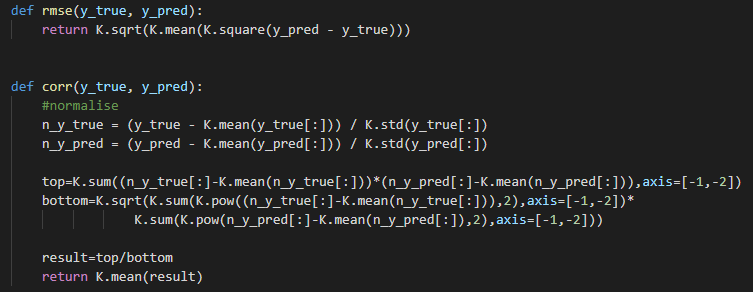
\includegraphics[angle=0, width=0.9\textwidth]{Figures/model_metrics.PNG}
  \caption{Model Custom Metrics}
  \label{fig:ModelCustomMetrics}
  \end{center}
\end{figure}


%%%%%%%%%%%%%%%%%%%%%%%%%%%%%%%%%%%%%%%%%%%%%%%%%%%%%%%
\section{Regularization}
A central role in developing a successful solution with Machine Learning is making sure that an algorithm will perform well not only on the training data, but also on previously unseen data. In many Machine Learning challenges it is common, that a well performing algorithm on the training data performs bad on previously-unseen data. This behaviour is called 'overfitting'. Strategies explicitly designed for decreasing overfitting, even at the expense of increasing the training error, are known as regularization. \citep{Goodfellow:2016:DeepLearning}
\newline\newline
In order to prevent overfitting and generalize a model better, \citet{Chollet:2017:DeepLearningPython} highlighted that the best solution is to get more training data, because the more a model is exposed to data, the lower the chance that it would overfit. However, when it is not possible to expose the model to more data, \citet{Chollet:2017:DeepLearningPython} recommended utilizing regularization techniques, which will force the model to focus on the most prominent patterns. These techniques constrain a model in a way that it can only store a certain amount or a certain type of information. According to \citet{Chollet:2017:DeepLearningPython}, the easiest way to prevent overfitting is to reduce the network's size, or in other words, to remove features. As a result, the number of trainable parameters in the model is reduced and thus, the model's capacity shrinks.

\subsubsection{Feature removal}
For the here proposed Machine Learning model it was not possible to increase the amount of training data, as this would make an objective comparison with benchmark paper impossible. Thus, further regularization techniques were applied. The first choice was also to reduce the network's size. The pre-trained VGGFace network already provides a big stack of layers that cannot be removed without losing valuable information. Therefore, the custom layers were reduced to a single Dense layer, which was proposed in a similar way by \citet{Pittaras:2017:FineTuningStrategiesComparison}.

\subsubsection{Dropout}
According to \citet{Chollet:2017:DeepLearningPython}, Dropout is one of the most effective and commonly used regularization techniques. When applied, noise is introduced during training by randomly setting a certain percentage of the layer's output values to zero. The Dropout applied in the proposed architecture was determined through extensive experimentation and was applied before and after the single Dense layer with a rate of 0.7 and 0.6 respectively. The following figure shows an example with a dropout rate of 0.5.

\begin{figure}[H]
  \begin{center}
  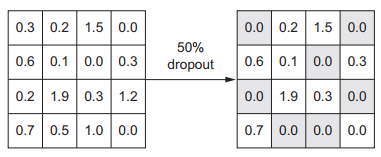
\includegraphics[angle=0, width=0.7\textwidth]{Figures/dropout.PNG}
  \caption{Dropout applied to an activation matrix at training time.\citep{Chollet:2017:DeepLearningPython}}
  \label{fig:Dropout}
  \end{center}
\end{figure}

\subsubsection{Data Augmentation}
Data Augmentation is another technique that is used to increase noise during training by randomly transforming existing training samples into slightly different looking images. As \citet{Chollet:2017:DeepLearningPython} argued that Data Augmentation exposes the model to more aspects of the data, as it will never see the exact same picture twice. As a result, the model will generalize better.
The Data Augmentation applied in the here proposed solution augmented the images randomly with the following parameters:

\begin{itemize}
    \item rotation range from 0 to 30 degrees
    \item width shift range from 0 to 25 percent of the total width
    \item height shift range from 0 to 25 percent of the total width
    \item horizontal flip
    \item brightness shift range from 50 to 150 percent
    \item zoom range from 0 to 30 percent
\end{itemize}


\subsubsection{Early Stopping}
Early Stopping is a callback that can be injected into the learning process of the Machine Learning model. Instead of running the training for a specified number of epochs, the Early Stopping callback can define a different criterion for the model to stop early. In the case of the here proposed solution, the Early Stopping callback monitored the validation loss metric. It stopped training 20 consecutive epochs after the last improvement on the validation loss was observed. The definition of this callback looks like this:

\begin{figure}[H]
  \begin{center}
  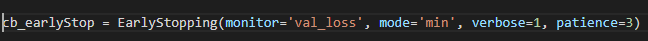
\includegraphics[angle=0, width=0.8\textwidth]{Figures/EarlyStopping.PNG}
  \caption{Early Stopping Callback}
  \label{fig:EarlyStopping}
  \end{center}
\end{figure}

The Early Stopping callback was combined with a Model Checkpoint callback that kept track of the best model during training and saved it to a predefined destination. The Model Checkpoint callback in the proposed solution also monitored the validation loss, and saved the current weights of the model at the point of the validation loss being the lowest. The definition of this callback loss looks like this:

\begin{figure}[H]
  \begin{center}
  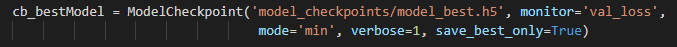
\includegraphics[angle=0, width=0.8\textwidth]{Figures/ModelCheckpoint.PNG}
  \caption{Model Checkpoint Callback}
  \label{fig:ModelCheckpoint}
  \end{center}
\end{figure}

To sum things up, the Model Checkpoint kept track of the currently best result in terms of reducing validation loss and automatically backed up the model's weights for the latest 'best result'. The Early Stopping Checkpoint interrupted training as soon as there was no improvement for 20 consecutive epochs.

\subsubsection{Hyper-parameter optimization}
Optimization of important hyper-parameters also greatly reduces the effects of overfitting. Two of the most impactful parameters are the learning rate and the batch size.
\newline\newline
An analysis conducted by \citet{Yuanzhi:2019:RegularizationInitialLargeLearningRate} on Initial Learning Rates confirmed that an initially large learning rate can have a regularization effect on the training process. Even though a small initial learning rate might allow for better performance initially, it will not be able to generalize as well as initially large learning rates. The training performed in this Master's thesis made use of an initial learning rate of 0.0001 for the first 3 epochs. Afterwards it was lowered down to 0.00001.
\newline\newline
Along with the effects of the initial learning rate on improving generalization and reducing the effects of overfitting, \citet{Keskar:2016:LargeBatchTrainingGeneralization} posited that choosing small-batch methods consistently generalize better than large batch methods. 
\newline\newline
To sum everything up, both the learning rate and batch size can offer a regularizing effect due to the noise they add during the training process.
